\documentclass[11pt]{beamer}

\usetheme{Warsaw}
\usepackage{relsize}
\usepackage[utf8]{inputenc}
\usepackage{amsmath}
\usepackage{amsfonts}
\usepackage{amssymb}
\usepackage{graphicx}
\usepackage{animate}
\usepackage{subfig}
\usepackage{color}
\usepackage{tikz}
\usepackage{coffee4}

\usepackage{dirtytalk}


%\author{}
%\title{}
%\setbeamercovered{transparent} 
%\setbeamertemplate{navigation symbols}{} 
%\logo{} 
%\institute{} 
%\date{} 
%\subject{}

\usepackage{hyperref}

\hypersetup{
	pdftex,
	pdfauthor={Guillermo Mosse},
	pdftitle={¡Qué colgado!},
	pdfsubject={Un acertijo matemático sobre topología (el grupo fundamental del plano pinchado)},
	pdfkeywords={grupo fundamental, pi1, topología, segundaria, estudiantes, acertijo, matemática, clavos, cuadro, semana de la matemática, Universidad de Buenos Aires, 2018}
}

 
\begin{document}

\title{¡Qué colgado!}
\date{Semana de la Matemática 2018}
\author{Billy - billy.mosse@gmail.com}


\begin{frame}
\maketitle
\end{frame}

%\begin{frame}
%\tableofcontents
%\end{frame}

\begin{frame}{Problema}

	Estoy aburrido en mi casa.
	\bigskip
	
	\visible<2->{Tengo un cuadro que quiero colgar de dos clavos.}
	\bigskip
	
	\visible<3->{Quiero que quede bien colgado.}
	\bigskip
	
	\visible<4->{PERO que si saco cualquiera de los dos clavos el cuadro se caiga.}
	
	\visible<5->{¿Por qué? Porque pintó.}
	
\end{frame}

\begin{frame}{para mí no}
	\huge{¿Se podrá?}
\end{frame}


\begin{frame}{Bueno, haciendo trampa sí}
	\center{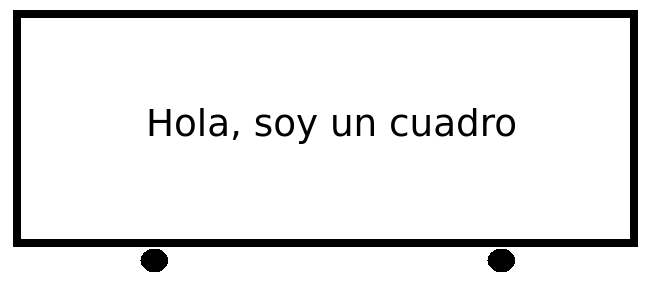
\includegraphics[scale=0.5]{images/soltrivial.png}}
	
\end{frame}

\begin{frame}{Uh así no vale}

%Esto no anda
%\animategraphics[height=2.8in,autoplay,controls]{12}{gifs/animate_}{0}{120}

\huge{¡Hay que definir bien el problema!}

\end{frame}


\begin{frame}{Empecemos de nuevo}

\begin{itemize}
	\item El cuadro tiene que estar abajo de los clavos
	\item Los clavos están fijos
	\visible<2->{\item La cuerda debe salir del cuadro y volver al cuadro}
	\bigskip
	\bigskip
		
	\visible<3->{\LARGE Las condiciones son ideales:}
	\bigskip
	\visible<3->{\normalsize \item La cuerda es irrompible}
	\visible<3->{\item No hay rozamiento (la cuerda no se traba)}
\end{itemize}

\visible<4->{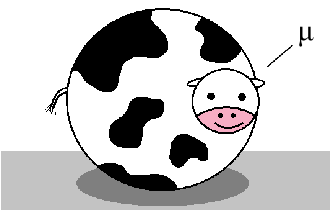
\includegraphics[scale=0.7]{images/cow.png}}

\end{frame}


\begin{frame}{Configuración usual}
	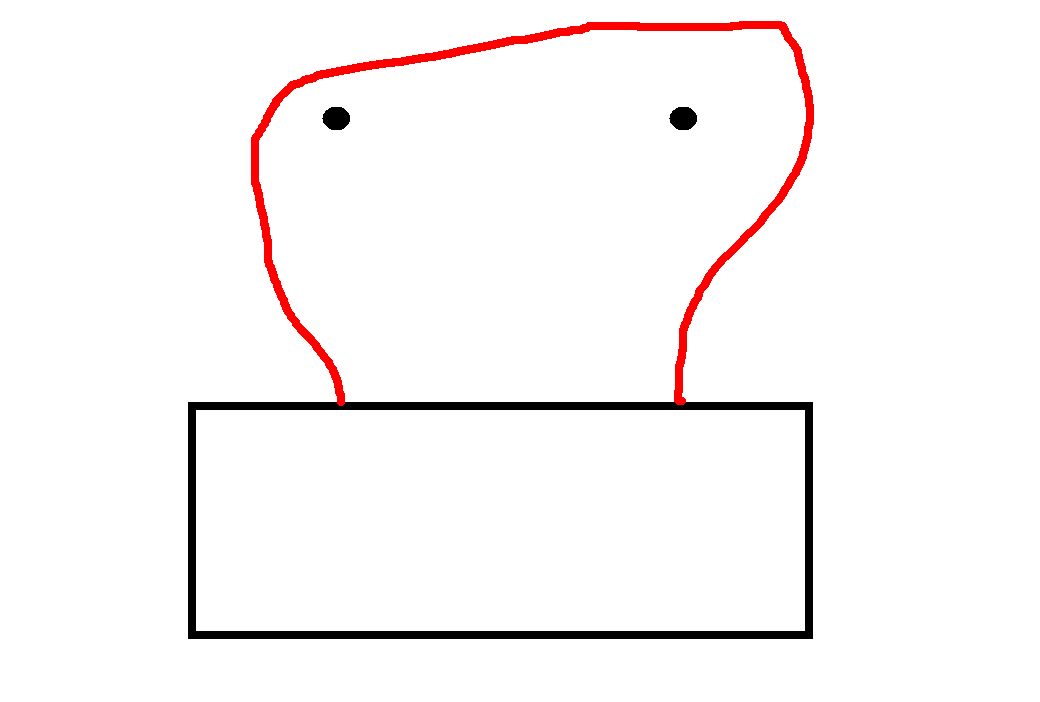
\includegraphics[scale=0.35]{images/xy_without.png}
	
	\visible<2->{Esta no anda.}
	
%		\begin{tikzpicture}[remember picture,overlay]
%    \node[xshift=-0.5cm,yshift=1.5cm] at (current page.south east)	%{
\includegraphics[scale=0.15]{images/vaca.png}};
%	\end{tikzpicture}
\end{frame}

\begin{frame}{Otra}
	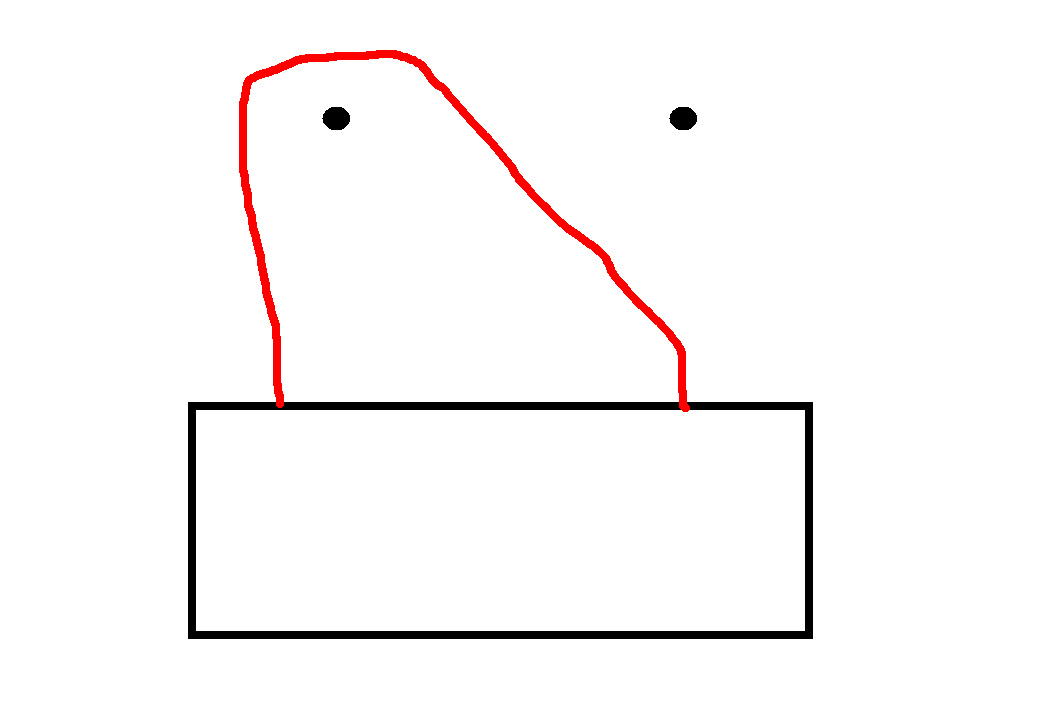
\includegraphics[scale=0.4]{images/x_without.png}
	
	\visible<2->{Esta tampoco. ¿Por qué?}
\end{frame}

\begin{frame}{Una rara}
	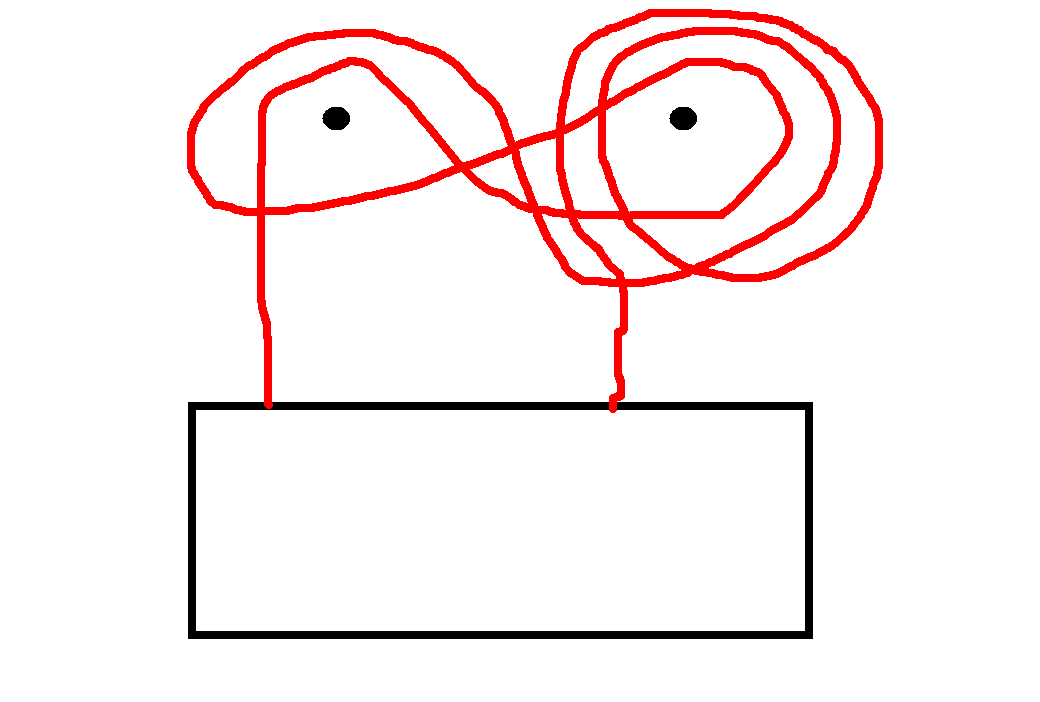
\includegraphics[scale=0.4]{images/config3.png}
	
	\visible<2->{Esta ni idea}
	
	%Esto motiva la idea de las fórmulas
	
%	\begin{tikzpicture}[remember picture,overlay]
%    \node[xshift=-0.5cm,yshift=1.5cm] at (current page.south east)	%{
\includegraphics[scale=0.15]{images/vaca2.png}};
%	\end{tikzpicture}
	
\end{frame}


\begin{frame}{Tratemos de entender esas curvas locas}

	Hay un montón de maneras de colgar un cuadro (¿cuántas hay?)
	
	¿Cómo entenderlas y estudiarlas? ¿Cómo chequear si son solución?
%	
%	\begin{figure}%
%    \centering
%    \subfloat{{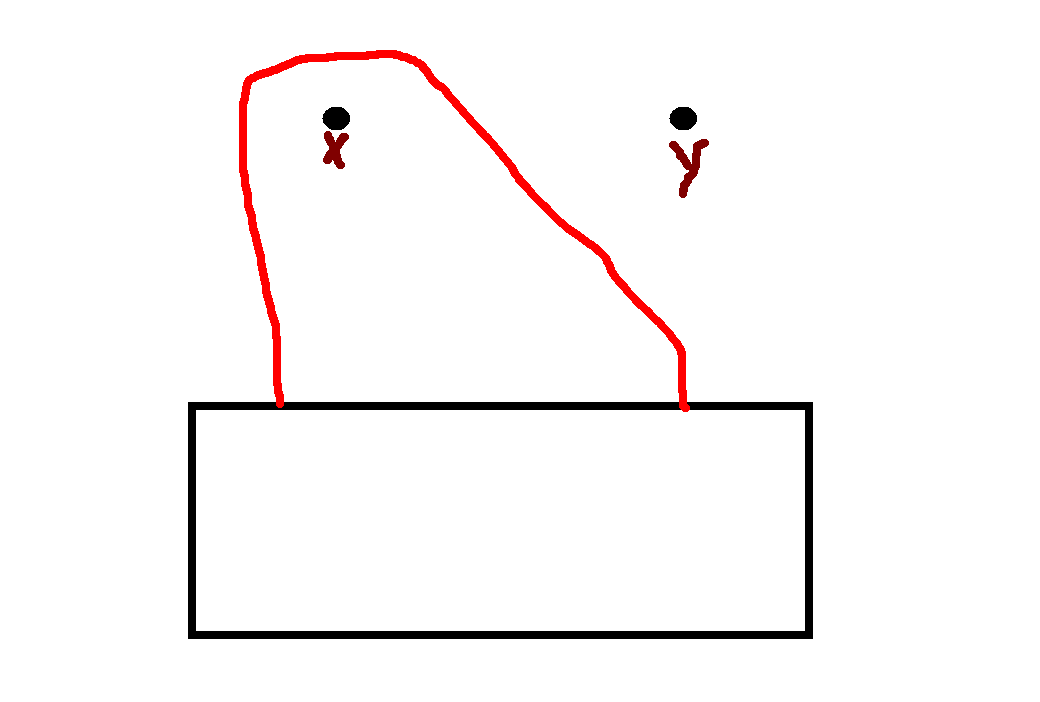
\includegraphics[width=5cm]{images/x.png} }}%
%    \qquad
%	\visible<2->{\subfloat{{\includegraphics[width=5cm]{images/y.png} }}%
%	}
%\end{figure}
%	

	\visible<2->{\Large{¡Poniéndoles nombres a las cosas!}}
	\visible<2->{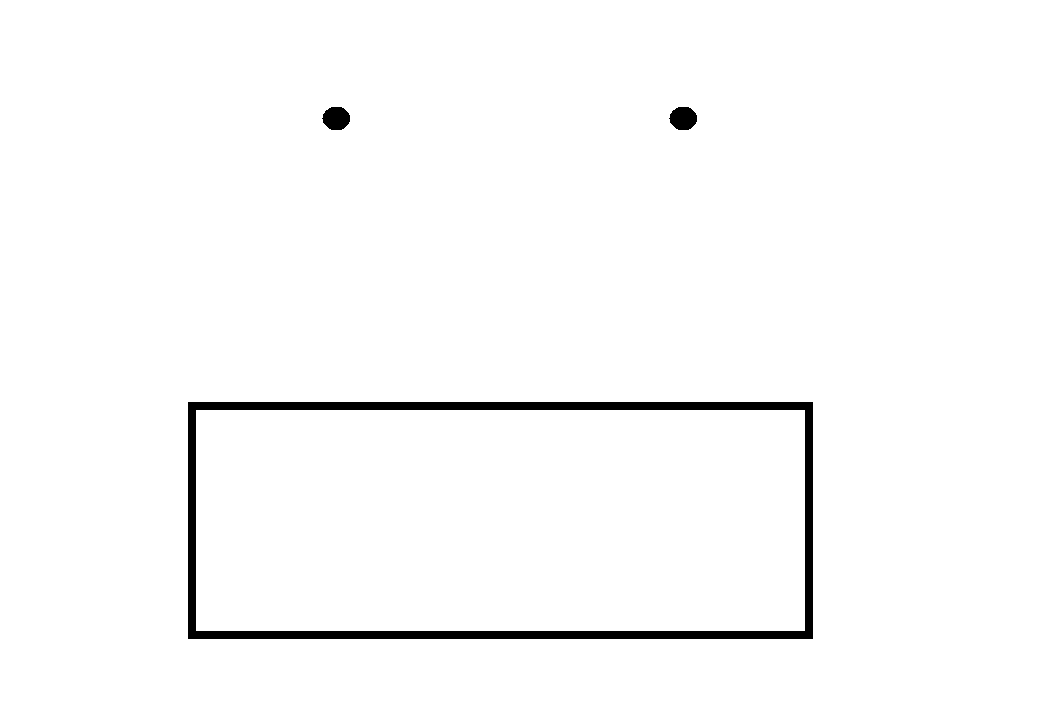
\includegraphics[scale=0.35]{images/basico.png}}

\end{frame}

\begin{frame}{Tratemos de entender esas curvas locas}

	Hay un montón de maneras de colgar un cuadro (¿cuántas hay?)
	
	¿Cómo entenderlas y estudiarlas? ¿Cómo chequear si son solución?


	\Large{¡Poniéndoles nombres a las cosas!}
	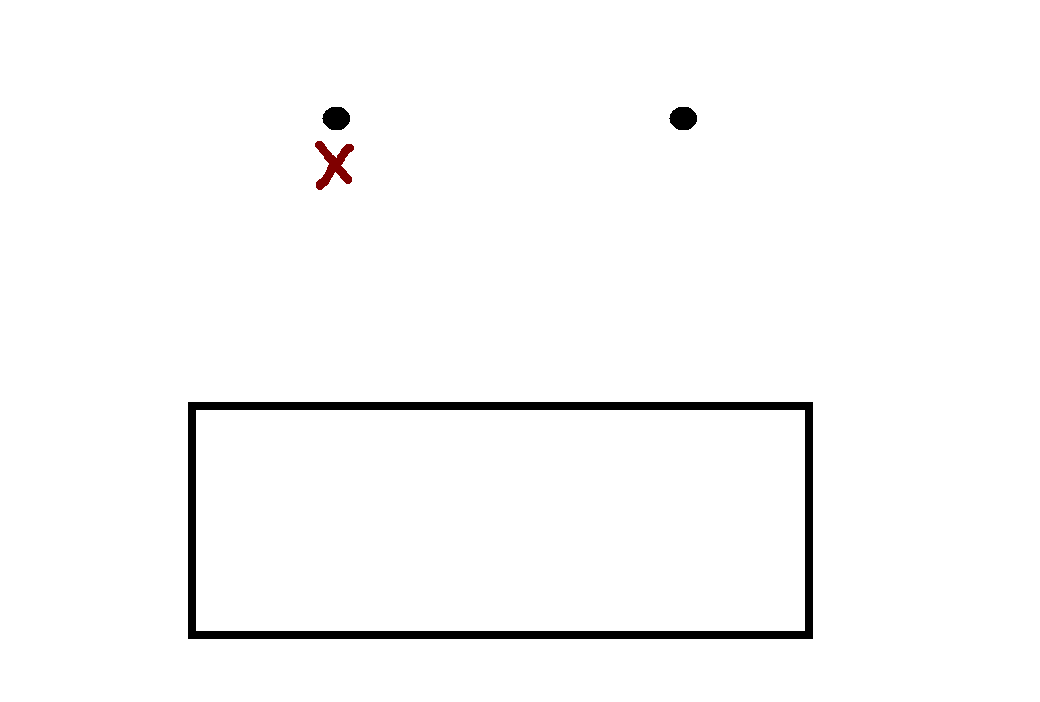
\includegraphics[scale=0.35]{images/_x.png}

\end{frame}

\begin{frame}{Tratemos de entender esas curvas locas}

	Hay un montón de maneras de colgar un cuadro (¿cuántas hay?)
	
	¿Cómo entenderlas y estudiarlas? ¿Cómo chequear si son solución?


	\Large{¡Poniéndoles nombres a las cosas!}
	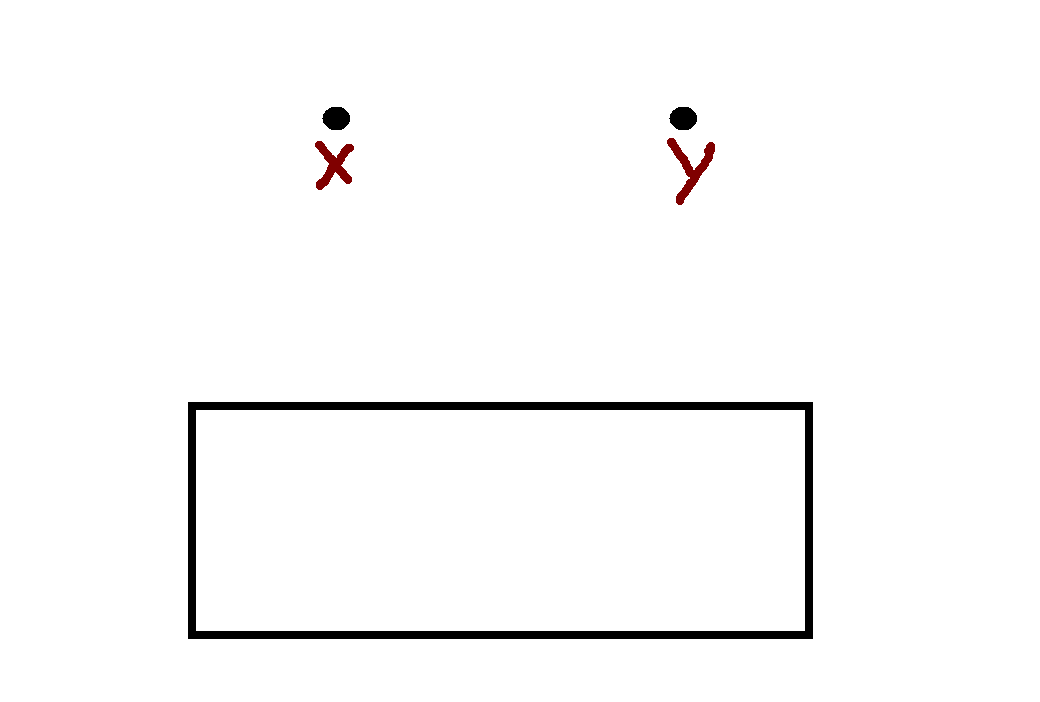
\includegraphics[scale=0.35]{images/_xy.png}

\end{frame}

% Ir por abajo no cambia nada
% Ir por arriba sí, porque "traba"
% Y no es lo mismo ir de izquierda a derecha que de derecha a izquierda

\begin{frame}{Curva $\rightarrow$ formulita}
	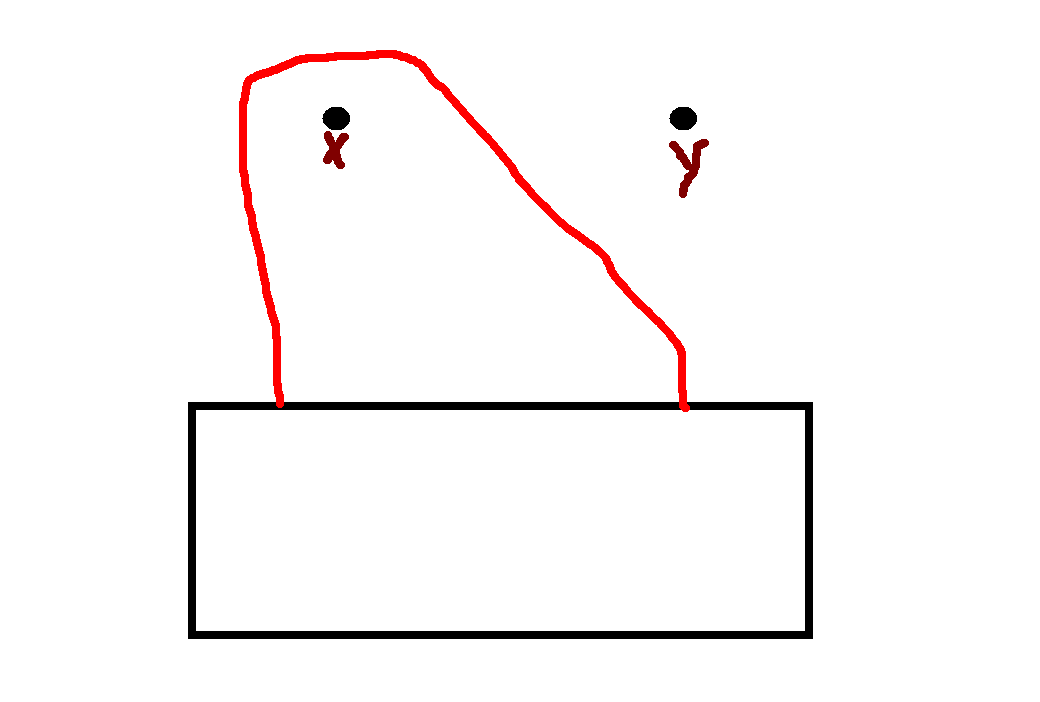
\includegraphics[scale=0.35]{images/x.png}
	
	
	Estamos pasando por arriba del clavo $x$.

	\visible<2->{\center{Nombre de la config: \color{red} \Huge{x}}}	

\end{frame}


\begin{frame}{Curva $\rightarrow$ formulita}
	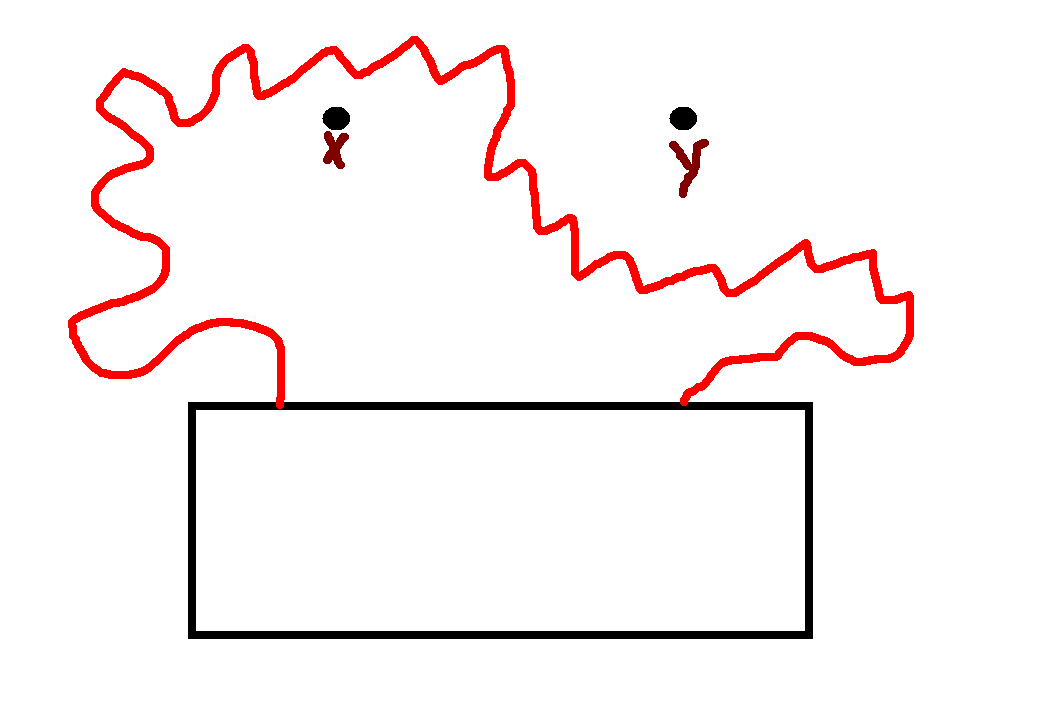
\includegraphics[scale=0.35]{images/x_v2.png}
	
	
	Esta, ¿qué nombre merece?

	\visible<2->{\center{Nombre de la config: \color{red} \Huge{x}}}	
	
\end{frame}

\begin{frame}{Distinción}
	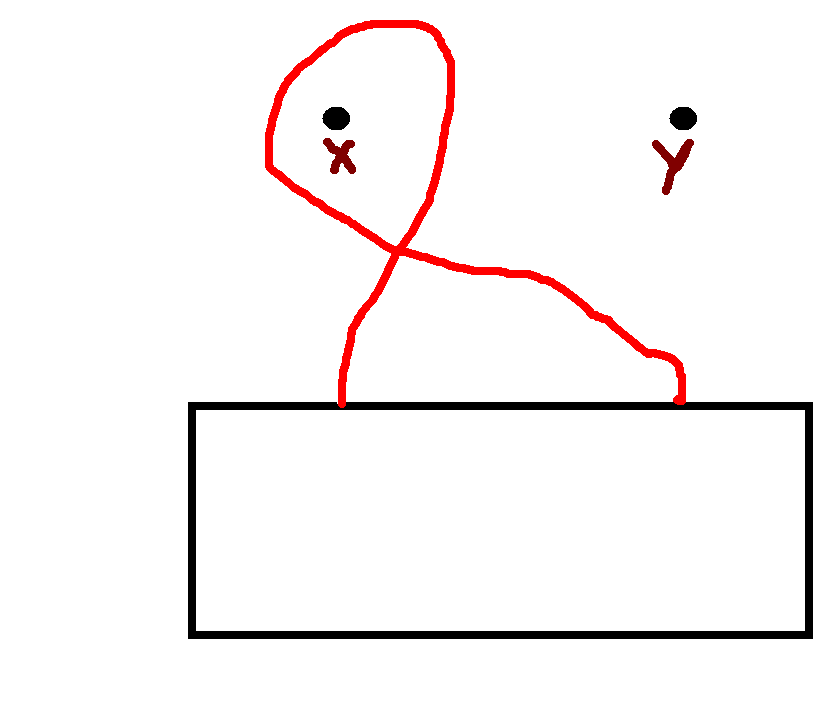
\includegraphics[scale=0.30]{images/x-1.png}

	%el 1 es demasiado grande
	En vez de ir de izquierda a derecha por arriba de x, estoy yendo de derecha a izquierda. \say{Al revés} 	\visible<2->{\color{red} \center{\Huge{$-x$}}}
	
\end{frame}

\begin{frame}{Curva $\rightarrow$ formulita}
	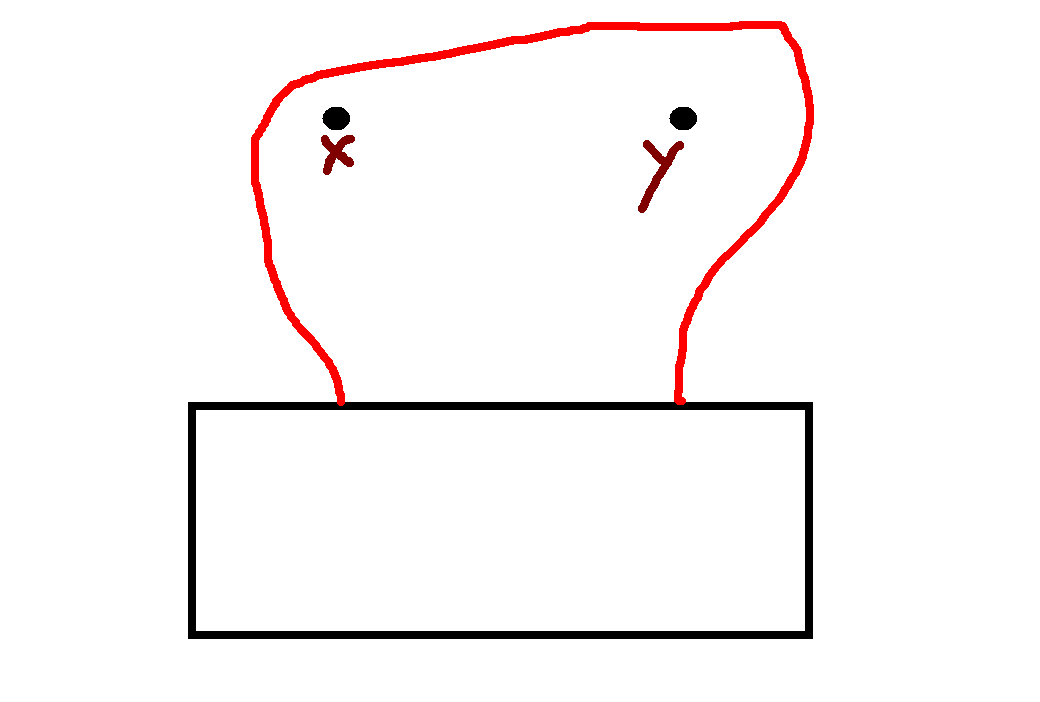
\includegraphics[scale=0.35]{images/xy.png}
	
	Estamos pasando por arriba del clavo $x$ y del clavo $y$.
	
	\visible<2->{ \center{Nombre de la config: \color{red} \Huge{x $+$ y}}}
	

\end{frame}

\begin{frame}{Curva $\rightarrow$ formulita}
	
	\color{red} \center{\Huge{y $+$ x}}
	
	\visible<2->{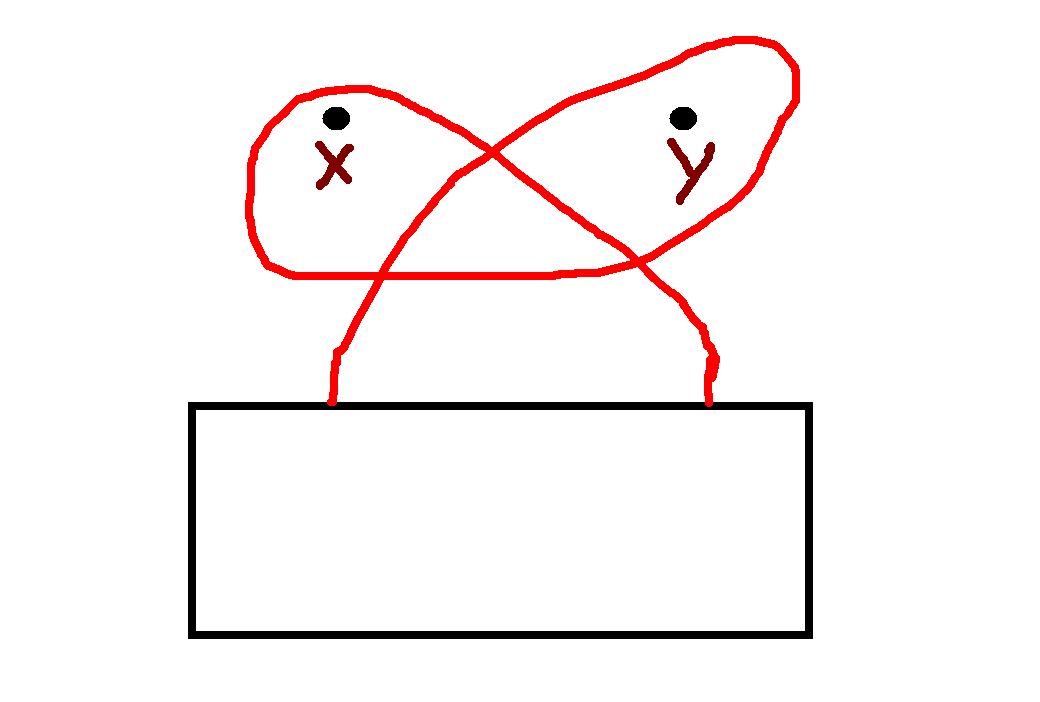
\includegraphics[scale=0.35]{images/yx.png}}
	
	\color{black} \visible<2->{"Ir por abajo no hace nada"}
	
\end{frame}


%tengo que decir que es x por x a la menos 1
\begin{frame}{¿Qué es el 0?}
\center{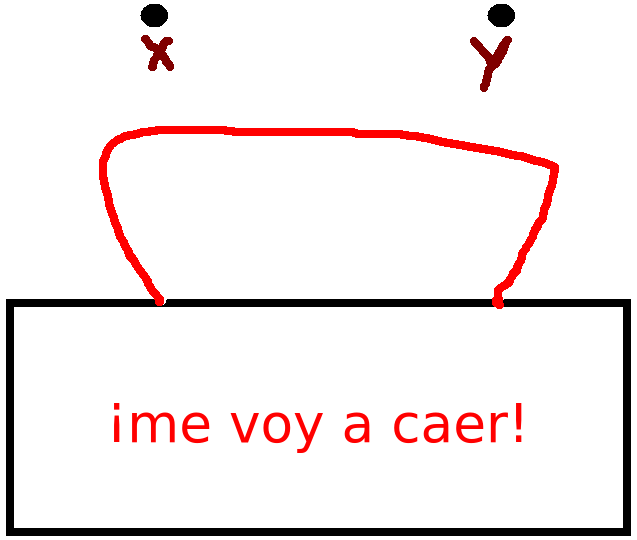
\includegraphics[scale=0.21]{images/1.png} }
	
\bigskip
\bigskip
\center{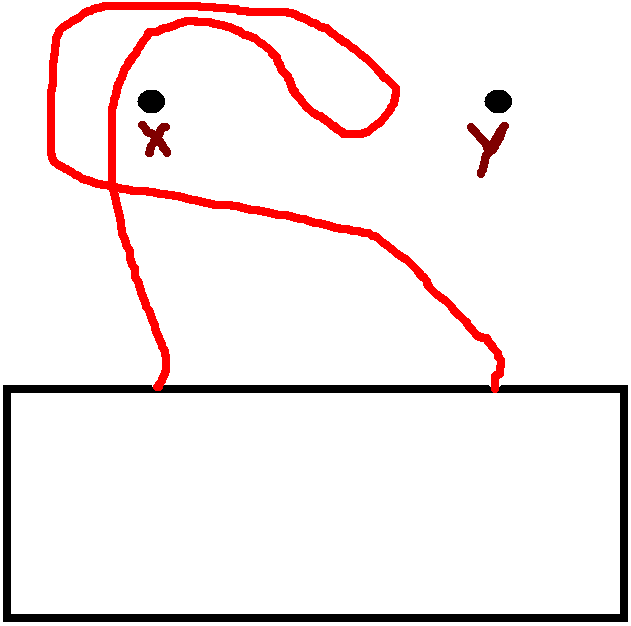
\includegraphics[scale=0.21]{images/xx-1.png}}

% Esto nos motiva a decir que x * x^{-1} = 1$ (ES uno)

% O sea, es lo mismo que on hacer nada

% Menciono clases de equivalencia?

% A veces uno cuando estudia objetos, dice que son iguales o equivalentes y deja de distinguirlos

% Esto con los numeros no pasaba!

\end{frame}


\begin{frame}{¿Qué es el 0?}
\center{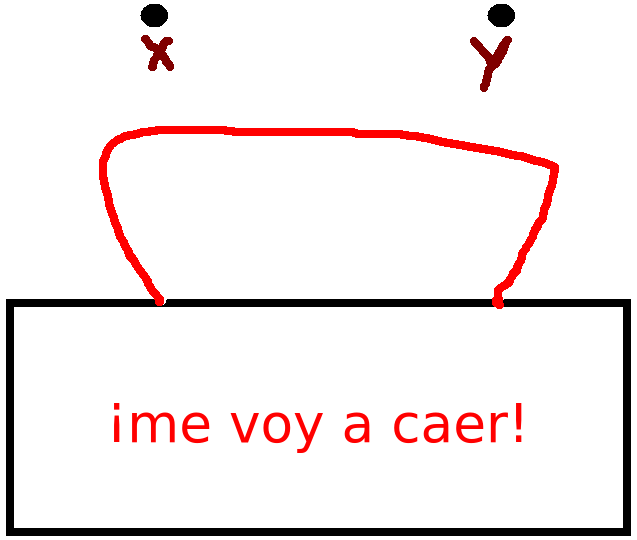
\includegraphics[scale=0.21]{images/1.png} }
	
\center{\scalebox{1.8}{$\equiv$}}


\center{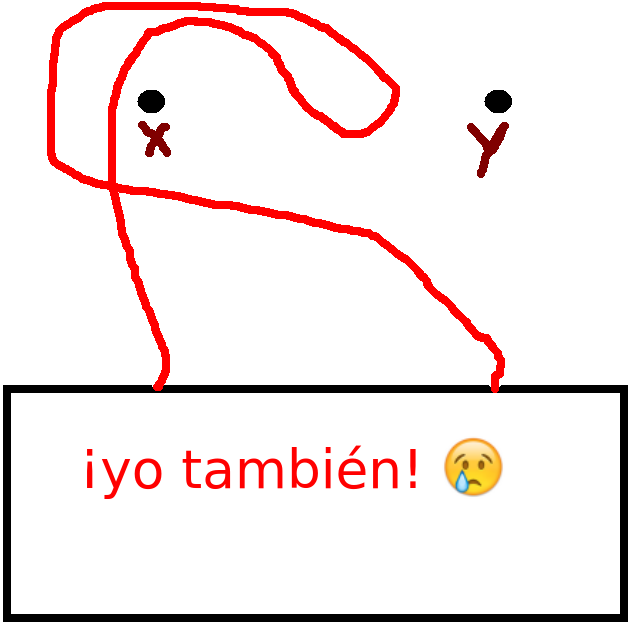
\includegraphics[scale=0.21]{images/xx-1_crying.png}}

% Esto nos motiva a decir que x * x^{-1} = 1$ (ES uno)

% O sea, es lo mismo que on hacer nada

% Menciono clases de equivalencia?

% A veces uno cuando estudia objetos, dice que son iguales o equivalentes y deja de distinguirlos

% Esto con los numeros no pasaba!

\end{frame}


\begin{frame}{Más ejemplos}

\bigskip

\bigskip

\center {\textbf {  \huge{[Pizarrón]}}}



%\hfill{{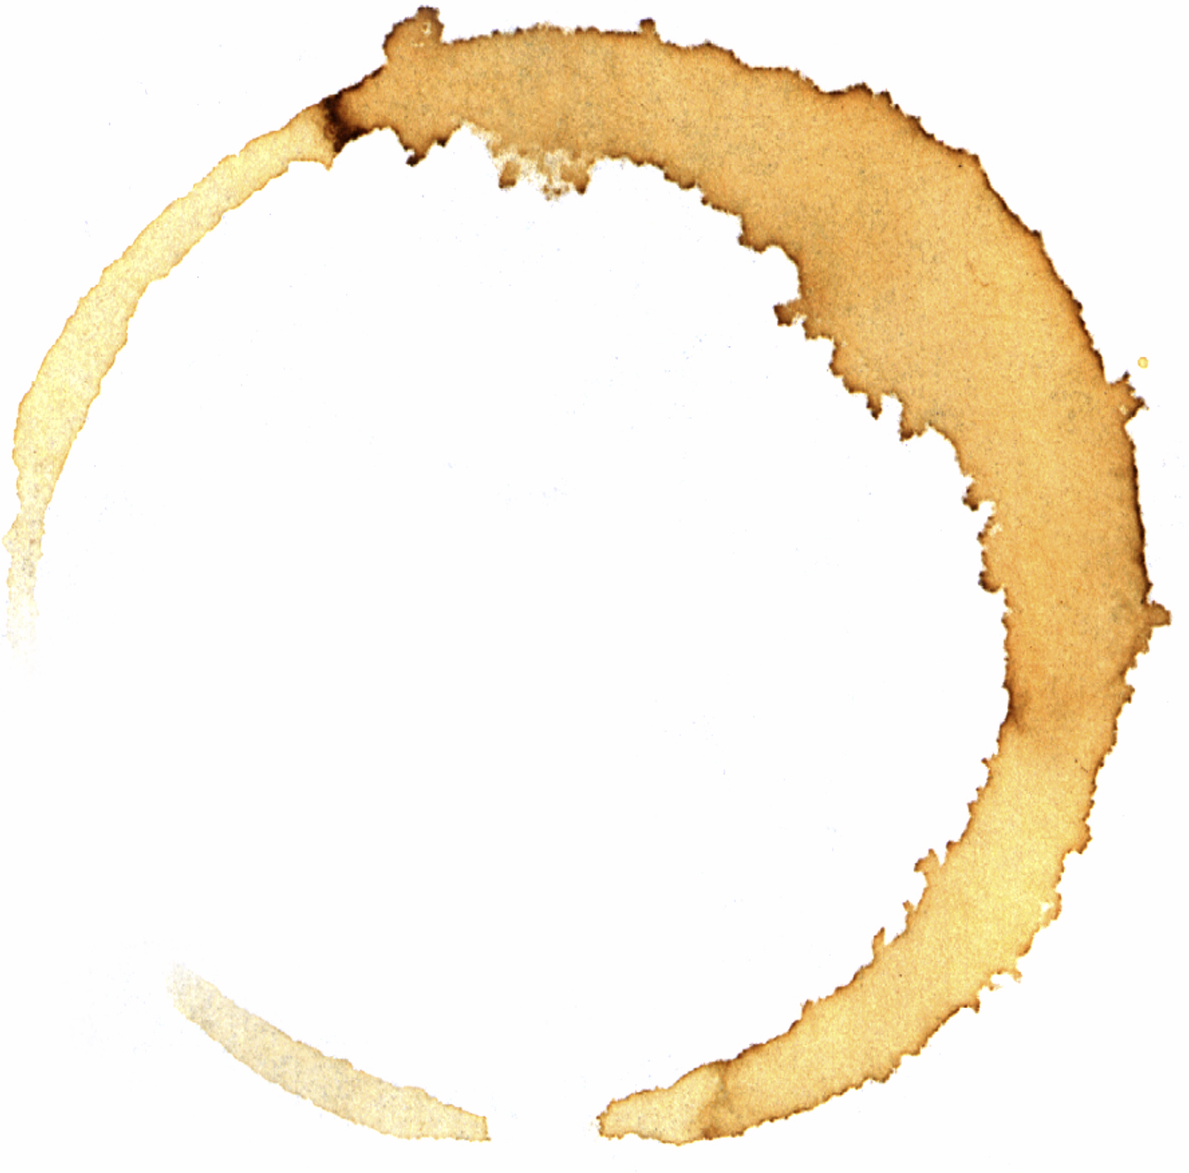
\includegraphics[scale=0.3]{images/coffee.png}}}


\cofeAm{0.4}{0.4}{0}{3cm}{1cm}

% Podríamos ver el ejemplo horrible del principio

% HACER EJEMPLO NO CONMUTATIVO XYX^-1

\end{frame}


\begin{frame}{¿Qué queremos? ¿Qué fórmula tiene?}

%TODO por que no sirven
Ya entendimos que {\color{red}$x$} no sirve, {\color{red}$-x$} tampoco. {\color{red}$0$} mucho menos.

% Estamos pudiendo representar cosas de la vida real con letras!

¿Cuál fórmula "servirá"?

\end{frame}


\begin{frame}{¿Qué significa "sacar un clavo"?}

Supongamos que tenemos el cuadro colgado como {\color{red}$x + y + x$}

¿Qué significa sacar el clavo $y$?

\bigskip

\visible<2>{\center{\Large{¡No les voy a decir la respuesta! Pensemos un toque.}}}

\visible<3>{\center{\Large{¡Desaparece la letra!}}}

\end{frame}





%TODO poner una mascota chiquita: eso significa ESPERA que sino quemas la respuesta.
%TODO armadillo, reloj. Armadillo de brazos cruzados es esperar, emocionado es segui

\begin{frame}{¿Qué había que hacer?}

¿Qué queremos?
\visible<2->{Queremos una fórmula que no sea equivalente a 0 pero cuando saco cualquiera de las dos letras, sí.}
\bigskip
%\visible<3->{Fíjense: $x -x = 0$. Ídem con $y$}


%\visible<3->{¿Cuándo lo queremos?}

\end{frame}

\begin{frame}{¿Qué queremos?}
\center \Huge{Pensemos un poco...}
\end{frame}

\begin{frame}{dale decime la solución}
\center \Huge{No, dale, en serio, pensemos...}
\end{frame}


\begin{frame}{Solución}

\center{\scalebox{2.5}{$x + y - x - y$}}

\bigskip

\bigskip

\visible<2->{\scalebox{2.5}{¿Es única?}}


\end{frame}

\begin{frame}{¿Y con más clavos?}

\center{\Huge{¿Qué pasa si tengo más clavos? Ahora hay 3: $x,y,z$}}

\bigskip

\center{\huge{¿Se podrá?}}

\end{frame}


\begin{frame}{Inducción}

\LARGE{Tenemos la solución para el caso $n=2$, y si tenemos una solución para $n$ clavos, podemos armar una solución para $n+1$ clavos.


% Me salió un verso sin esfuerzo
Entonces,  ¡siempre hay solución! A este tipo de razonamiento lo llaman hacer inducción.

\bigskip

\visible<2->{Y eso está buenísimo, porque las demostraciones inductivas suelen ser fáciles de programar\textsuperscript{[cita requerida]}}}


\visible<3->{\center{¿Cuánto se va complejizando la solución? ¿Cuántas multiplicaciones hay que hacer?}}


\end{frame}


%xkcd induction

%Podes hacer animacion, graficando.

\begin{frame}{Programita}
\huge\center{Miren esto!}
\end{frame}

\begin{frame}
		\huge{¿Preguntas?} 
		
		\bigskip
		\LARGE{¿Comentarios?}
		
		\bigskip
		\large{¿Sugerencias?}
		
		\bigskip
		\normalsize{¿Expresiones de asombro?}
		
		\bigskip
		\footnotesize {¿Alguno más quiere una \\
		 mejor compu para ver qué\\
		 pasa cuando n = 3000?}
		 
		 \bigskip
		 
		 \tiny{¿Alguno más tiene hambre?}
%				\begin{tikzpicture}[remember picture,overlay]
%    \node[xshift=-2.1cm,yshift=-5.6cm] %at (current page.north east) %{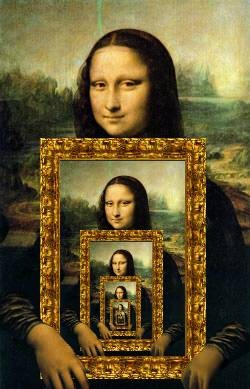
\includegraphics[scale=1.12]{images/monalisa.jpg}};
%	\end{tikzpicture}

				\begin{tikzpicture}[remember picture,overlay]
    \node[xshift=-3.8cm,yshift=-4.6cm] at (current page.north east) {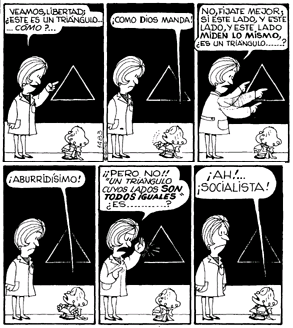
\includegraphics[scale=0.72]{images/triangulo.png}};
	\end{tikzpicture}


\end{frame}

\end{document}